%%%%%%%%%%%%%%%%%%%%%%%%%%%%%%%%%%%%%%%%%
% University/School Laboratory Report
% LaTeX Template
% Version 3.1 (25/3/14)
%
% This template has been downloaded from:
% http://www.LaTeXTemplates.com
%
% Original author:
% Linux and Unix Users Group at Virginia Tech Wiki 
% (https://vtluug.org/wiki/Example_LaTeX_chem_lab_report)
%
% License:
% CC BY-NC-SA 3.0 (http://creativecommons.org/licenses/by-nc-sa/3.0/)
%
%%%%%%%%%%%%%%%%%%%%%%%%%%%%%%%%%%%%%%%%%

%----------------------------------------------------------------------------------------
%	PACKAGES AND DOCUMENT CONFIGURATIONS
%----------------------------------------------------------------------------------------

\documentclass{article}

%\usepackage[version=3]{mhchem} % Package for chemical equation typesetting
%\usepackage{siunitx} % Provides the \SI{}{} and \si{} command for typesetting SI units
\usepackage{graphicx} % Required for the inclusion of images
\usepackage[section]{placeins}
\usepackage{booktabs}
%\usepackage{natbib} % Required to change bibliography style to APA
%\usepackage{amsmath} % Required for some math elements 

\setlength\parindent{0pt} % Removes all indentation from paragraphs

\renewcommand{\labelenumi}{\alph{enumi}.} % Make numbering in the enumerate environment by letter rather than number (e.g. section 6)

%\usepackage{times} % Uncomment to use the Times New Roman font

%----------------------------------------------------------------------------------------
%	DOCUMENT INFORMATION
%----------------------------------------------------------------------------------------

\title{Overview of RNA-seq reads for \textit{Eimeria falciformis} and \textit{Mus musculus}} % Title

\author{Totta \textsc{Kasemo}} % Author name

\date{\today} % Date for the report

\begin{document}

\maketitle % Insert the title, author and date

\begin{center}
\begin{tabular}{l r}
%Date Performed: & January 1, 2012 \\ % Date the experiment was performed
%Partners: & James Smith \\ % Partner names
%& Mary Smith \\
%Instructor: & Professor Smith % Instructor/supervisor
\end{tabular}
\end{center}

% If you wish to include an abstract, uncomment the lines below
% \begin{abstract}
% Abstract text
% \end{abstract}

%----------------------------------------------------------------------------------------
%	SECTION 1
%----------------------------------------------------------------------------------------

\section{Objective}

This summary table of reads generated in each sample.....

%\begin{center}\ce{}\end{center}

%----------------------------------------------------------------------------------------
%	SECTION 2 
%----------------------------------------------------------------------------------------

\section{Table of reads per sample}

% latex table generated in R 3.2.2 by xtable 1.8-2 package
% Wed Mar  2 14:36:30 2016
\begin{table}[ht]
\centering
\begin{tabular}{llll}
  \hline
Samples & Percent \emph{E. falciformis} & Mouse Transcripts & \emph{E. falciformis} Transcripts \\
  \hline
NMRI\_oocysts &  99.9854842 & 17516.000 & 120650726.000 \\
  NMRI\_sporozoites &  99.9805302 & 20860.000 & 107119299.000 \\
  NMRI\_1stInf\_7dpi\_rep1 &  83.5224277 & 18350269.000 & 93014856.000 \\
  NMRI\_1stInf\_7dpi\_rep2 &  54.9450408 & 145227236.000 & 177106284.000 \\
  NMRI\_2ndInf\_7dpi\_rep1 &   7.0575562 & 149369191.000 & 11342304.000 \\
  NMRI\_1stInf\_5dpi\_rep1 &   5.9692983 & 320787124.000 & 20364349.000 \\
  C57BL6\_1stInf\_5dpi\_rep2 &   0.5892196 & 46455447.000 & 275347.000 \\
  NMRI\_2ndInf\_5dpi\_rep1 &   0.4501036 & 917436287.000 & 4148084.000 \\
  NMRI\_1stInf\_5dpi\_rep2 &   0.3615460 & 490566909.000 & 1780061.000 \\
  C57BL6\_2ndInf\_5dpi\_rep1 &   0.3550692 & 95259948.000 & 339444.000 \\
  NMRI\_1stInf\_3dpi\_rep1 &   0.2721386 & 328870247.000 & 897425.000 \\
  C57BL6\_1stInf\_5dpi\_rep1 &   0.2347177 & 101231812.000 & 238168.000 \\
  Rag\_2ndInf\_5dpi\_rep1 &   0.1850507 & 132358804.000 & 245385.000 \\
  Rag\_1stInf\_5dpi\_rep2 &   0.1427648 & 88257677.000 & 126181.000 \\
  NMRI\_1stInf\_3dpi\_rep2 &   0.1216664 & 809232397.000 & 985763.000 \\
  Rag\_1stInf\_5dpi\_rep1 &   0.0712794 & 112174061.000 & 80014.000 \\
  NMRI\_2ndInf\_7dpi\_rep2 &   0.0271172 & 193993643.000 & 52620.000 \\
  NMRI\_2ndInf\_3dpi\_rep2 &   0.0235337 & 162464901.000 & 38243.000 \\
  NMRI\_1stInf\_0dpi\_rep1 &   0.0108286 & 347939504.000 & 37681.000 \\
  NMRI\_2ndInf\_5dpi\_rep2 &   0.0079426 & 178050386.000 & 14143.000 \\
  NMRI\_2ndInf\_3dpi\_rep1 &   0.0043015 & 142131560.000 & 6114.000 \\
  NMRI\_2ndInf\_0dpi\_rep2 &   0.0030853 & 140081531.000 & 4322.000 \\
  Rag\_1stInf\_0dpi\_rep1 &   0.0008362 & 67091135.000 & 561.000 \\
  Rag\_1stInf\_0dpi\_rep2 &   0.0007451 & 126286703.000 & 941.000 \\
  C57BL6\_1stInf\_0dpi\_rep1 &   0.0007381 & 82105133.000 & 606.000 \\
  C57BL6\_1stInf\_0dpi\_rep2 &   0.0006947 & 119614354.000 & 831.000 \\
  NMRI\_2ndInf\_0dpi\_rep1 &   0.0000834 & 441473116.000 & 368.000 \\
  
 
  \hline
\end{tabular}
\caption{Transcripts per sample listed for \textit{E. falciformis}, mouse and for the percentage of \textit{E. falciformis} transcripts out of the total (mouse plus parasite) transcripts. }
\end{table}

\section{Experimental overview with transcripts per sample}
	\setlength{\tabcolsep}{14pt}
\begin{table}
	\begin{center}
%\begin{tabular}{@{} *4l @{}}    \toprule
\begin{tabular}{*4l}    \toprule
\emph{Day, 1st infection}  	& NMRI  & C57BL/6  & Rag1-/- \\ \midrule
0 (control)     & $10^4$ / $10^8$  & $10^2$ / $10^8$  & $10^2$ / $10^7$  \\ %rep1/rep2, NA=no replicate
3  		& $10^5$ / $10^8$ & NA  & NA \\ 
5  		& $10^7$ / $10^8$ & $10^5$ / $10^7$  & $10^5$ / $10^8$ \\
7  		& $10^8$ / $10^7$ & NA  & NA \\ 
Oocysts 	& $10^8$ / NA & NA  & NA \\ 
Sporozoites 	& $10^8$ / NA & NA  & NA \\ \midrule

\emph{Day, 2nd infection}  	\\ \midrule
0 (control)     & $10^x$ / $10^x$  & $10^x$ / $10^x$  & $10^x$ / $10^x$  \\ %rep1/rep2, NA=no replicate
3  		& $10^x$ / $10^x$ & NA  & NA \\ 
5  		& $10^x$ / $10^x$ & $10^x$ / $10^x$  & $10^x$ / $10^x$ \\
7  		& $10^x$ / $10^x$ & NA  & NA \\ 
	
	
	\bottomrule
 \hline
\end{tabular}
	\caption{Transcripts numbers as order of magnitude for \emph{E. falciformis} (first) and mouse (second). Replicate average shown. For exact values, see ... . }
\end{center}
\end{table}

\section{Mouse RNA-seq data compared with mouse microarray data}
% figure 1
\begin{figure}[h]
\begin{center}
\includegraphics[width=0.8\textwidth]{~/Ef_RNAseq/figures/Array144_vs_RNAseqN7} % Merge 2 plots: RUV and non-RUV 
\caption{Comparison of mouse data from RNA-seq, day 7, (y-axis) and microarray data, day 6 (x-axis, (schmid14)). a. Data normalised with upperquartile method implemented in R package edgeR (version ...). $R^2$ = yy. b. Data adjusted with RUV method as implemented in R package RUVseq (version....). $R^2$ = xx. Each axis shows log fold changes on day 6 (microarray) and 7 (RNA-seq) post infection compared to control.}
\end{center}
\end{figure}

% figure 1
\begin{figure}[h]
\begin{center}
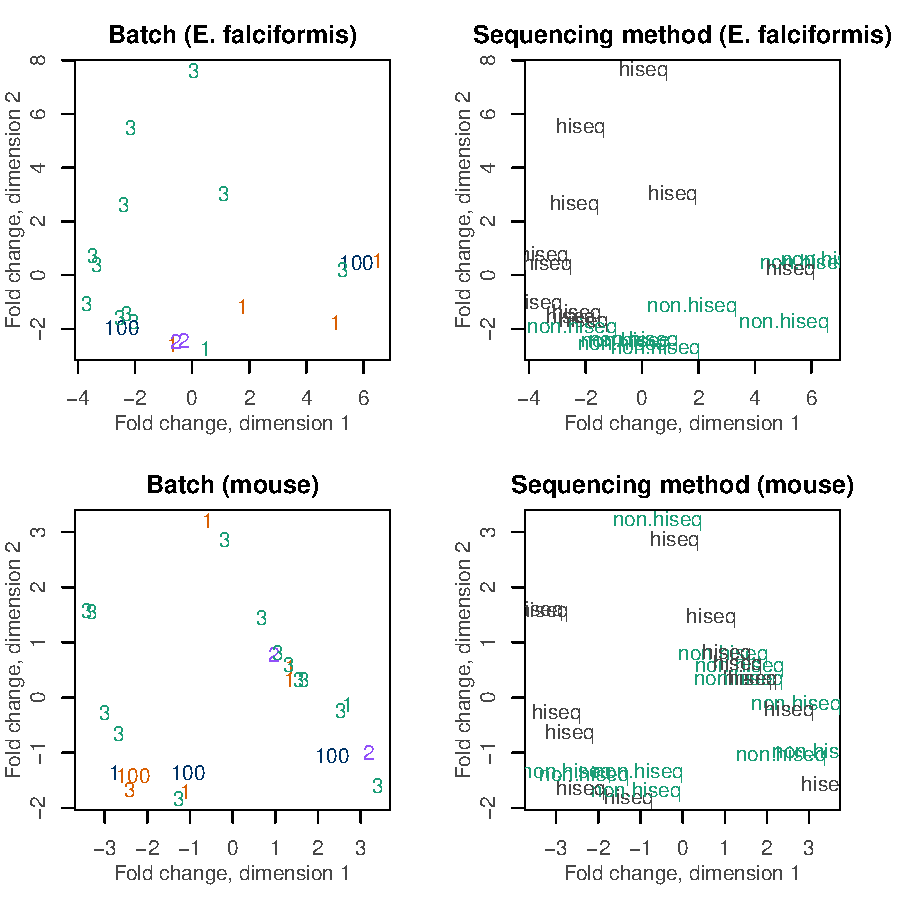
\includegraphics[width=0.8\textwidth]{~/Ef_RNAseq/figures//old_figures/EfMm_2mds} % Include 
	\caption{Multidimensional scaling shows no clear sample pattern due to technical variation. Samples shown with a. batch and b. sequencing method visualized for mouse (upper) and \emph{E. falciformis} (lower).}
\end{center}
\end{figure}

\end{document}

